\documentclass[10pt]{article}
\usepackage[margin=0.8in]{geometry}
\usepackage{amsmath,booktabs,hyperref,tikz,xcolor}
\hypersetup{colorlinks=true,urlcolor=blue,linkcolor=blue}
\definecolor{minimum}{HTML}{267C92}
\definecolor{higher}{HTML}{EF8F57}
\title{A Source-Verified Index of Odd-Characteristic Elliptic Covering Cases}
\author{Research note}
\date{12 October 2026}
\begin{document}
\maketitle
\noindent\textbf{Contribution.} The 36 numbered elliptic covering cases in
Iijima--Momose--Chao's 2015 classification are now queryable by extension degree
$d$, binary covering rank $n$, excess genus $e=g(C)-d$, and allowed coefficient
square class. Five cases have the minimum genus $g(C)=d$; 31 have larger genus.
This count is of published parameter families, not of exact elliptic models.
The source is \url{https://eprint.iacr.org/2015/805.pdf}, Section 5.

\begin{center}
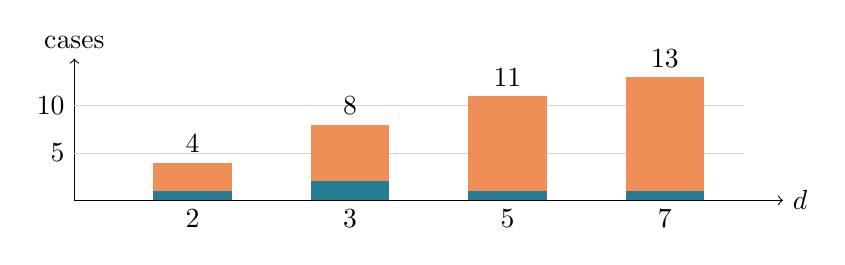
\begin{tikzpicture}[x=1cm,y=0.12cm]
\draw[->] (0,0)--(9,0) node[right] {$d$};
\draw[->] (0,0)--(0,15) node[above] {cases};
\foreach \y in {5,10} {\draw[gray!35] (0,\y)--(8.5,\y); \node[left] at (0,\y) {\y};}
\fill[minimum] (1,0) rectangle (2,1); \fill[higher] (1,1) rectangle (2,4);
\fill[minimum] (3,0) rectangle (4,2); \fill[higher] (3,2) rectangle (4,8);
\fill[minimum] (5,0) rectangle (6,1); \fill[higher] (5,1) rectangle (6,11);
\fill[minimum] (7,0) rectangle (8,1); \fill[higher] (7,1) rectangle (8,13);
\foreach \x/\d/\v in {1.5/2/4,3.5/3/8,5.5/5/11,7.5/7/13}
  {\node[below] at (\x,0) {$\d$}; \node[above] at (\x,\v) {\v};}
\end{tikzpicture}

\small\colorbox{minimum}{\strut\phantom{xx}} minimum genus $g(C)=d$ \quad
\colorbox{higher}{\strut\phantom{xx}} higher genus. Counts from 36 rows on
the paper's printed pages 17--18; one bar per degree.
\end{center}

\begin{center}
\begin{tabular}{rrrrr}\toprule
$d$ & cases & $g(C)=d$ & higher genus & largest $g(C)$\\\midrule
2&4&1&3&5\\
3&8&2&6&17\\
5&11&1&10&129\\
7&13&1&12&769\\\bottomrule
\end{tabular}
\end{center}

\noindent The five minimum-genus cases are paper Cases 1, 5, 6, 13, and 24.
The 2013 isogeny-condition list has 27 cases across elliptic and genus-two and
genus-three source curves; it has a different scope and overlaps this table
(\url{https://eprint.iacr.org/2013/487.pdf}).

\paragraph{Constructive screen.}
For $k=\mathbf F_q$ and $k_d=\mathbf F_{q^d}$, choose a listed binary factor
$F\mid X^d+1$ of degree $n$ and set $\widehat F=(X^d+1)/F$. The source's
Procedure 1 chooses $a$ coprime to $F$ and uses
$\Phi=a\widehat F\pmod{X^d+1}$ as a binary Frobenius ramification mask.
Cyclically rotated masks are equivalent. The native Rust replay records 27
mask orbits over the 11 listed factors. For the cubic $n=2$ branch,
$F=X^2+X+1$ and $\widehat F=X+1$, giving mask $011$ and roots
$\{\alpha,\alpha^q\}$. Case 5's source polynomial has four factors
$(x-\alpha_1)(x-\alpha_1^q)(x-\alpha_2)(x-\alpha_2^q)$;
the separate cubic $n=3$ minimum-genus branch is Case 6.

\begin{center}
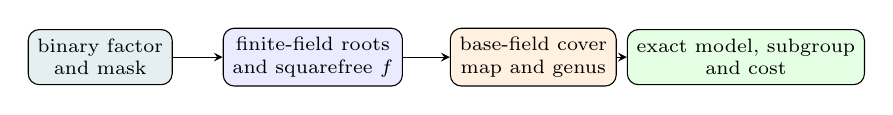
\begin{tikzpicture}[>=stealth, every node/.style={draw,rounded corners,align=center,font=\scriptsize,minimum height=0.7cm}]
\node[fill=minimum!12] (a) at (0,0) {binary factor\\and mask};
\node[fill=blue!8] (b) at (2.7,0) {finite-field roots\\and squarefree $f$};
\node[fill=orange!12] (c) at (5.5,0) {base-field cover\\map and genus};
\node[fill=green!10] (d) at (8.2,0) {exact model, subgroup\\and cost};
\draw[->] (a)--(b); \draw[->] (b)--(c); \draw[->] (c)--(d);
\end{tikzpicture}

\small Current native and Lean checks address the first gate; an exact curve
requires certificates for the later gates.
\end{center}

\noindent To realize a case, include every conjugate root over $k_d$, choose
a squarefree cubic or quartic $f$, enforce the paper's condition
$F(\sigma)f=1$ in $k_d(x)^*/k_d(x)^{*2}$, then verify the base-field model,
covering map, genus, exact twist, and selected-subgroup transport. A binary
mask by itself is a candidate. The two factorization identities for degrees
three and seven are Lean-checked with only standard Lean foundations;
formalizing the covering classification remains open. The accompanying
\texttt{REPORT.md}, \texttt{PROOF\_MAP.md}, and SQLite file record the source,
formalization status, and reproducible queries.

\paragraph{A checked negative discriminator.} Costa et al., Theorem 2.8
(\url{https://arxiv.org/pdf/2002.02067}), rules out a genus-three
hyperelliptic Jacobian when its second Weil coefficient is even and its
third is odd. A cubic restriction with polynomial
$T^6-tT^3+q^3$ meets that excluded pattern for odd $t$. Direct database
queries found zero odd traces in 87,486 complete exact ordinary rows and
246,512 ordinary cubic diagnostic rows. Thus this parity test separates none
of the unresolved rows in the current corpus; it addresses only the
hyperelliptic branch.
\end{document}
